\documentclass[12pt]{article}
\usepackage[utf8]{inputenc}
\usepackage{fancyhdr}
\usepackage{graphicx}
\usepackage{geometry}
\usepackage{float}
\usepackage[utf8]{inputenc}
 
\usepackage{array}
\usepackage{makecell}

% ---- Commands ------- %
\newcommand{\documentNumber}[1]{
    \LARGE  \textbf{ Processrapport }
    \\
    \medskip
}
\newcommand{\documentVersion}[1]{
    \medskip
}
\newcommand{\documentTitle}[1]{
    \centerline{\rule{13cm}{0.4pt}}
    \bigskip \bigskip
    \LARGE \textbf{Projekt IDA3} \\
    \bigskip
    \LARGE {#1} \\
    \bigskip \bigskip
    \centerline{\rule{13cm}{0.4pt}}
}

\newcommand{\documentDate}[1]{
    \date {#1} 
}

\renewcommand\theadalign{bc}
\renewcommand\theadfont{\bfseries}
\renewcommand\theadgape{\Gape[5pt]}
\renewcommand\cellgape{\Gape[5pt]}


\renewcommand{\contentsname}{Innehållsförtäckning}

% --- Header & Footer ---- %
\pagestyle{fancy}
\lhead{\leftmark}
\rhead{}
\rfoot{\thepage}
\cfoot{}
\lfoot{}


% ------------------------------------------------ #

% ----- FILL THIS ----- %
\title {
    \documentNumber {01}    

    % Full name - SHORTNAME
    \documentTitle {Helsingborg Event and Convention Bureau}
    
    % Format: YYYY-MM-DD
    \documentDate {2021-09-29}
    \documentVersion Vv 0.1
    
    \author{Anna Bergvall - Oscar Blixt - Pontus Persson - Filip Sjövall - David Vilppu - Sabah Zafar}
}

\begin{document}
\addtocontents{toc}{\protect\setcounter{tocdepth}{2}}
\maketitle

\thispagestyle{empty}



\newpage

\tableofcontents


\newpage

\section{Dokument Historia}
\begin{tabular}{ l | l | l }
    Version & Date & Description \\
    \hline
    0.1 & 2021-09-29 & Dokumentet skapat. Målbild och process. \\
    \hline
    0.2 & 2021-10-10 & Dokument uppdaterat med ändringar enligt anvisning. \\
    \hline
   
\end{tabular}

\newpage
% ----- SKRIV UNDER VARJE TITEL ----- %

\section{Målbild}
\subsection{Elevator Statement}


Vår målgrupp är kommuner och städer som önskar att gå med i det globala nätverket Global
Destination Sustainability Movement (GDSM). Som medlem i nätverket rapporteras det
årligen in hållbarhetsdata som bidrar till en positiv utveckling av staden som en mötes-och
evenemangsdestination. \\ \indent Sustainable Form är ett digitalt rapporteringsverktyg som samlar in
och sammanställer hållbarhetsdata från aktörer inom besöksnäring i städer och kommuner.
Till skillnad från Google Forms ger vår digitala rapporteringsverktyg skräddarsydd
sammanställning och större kontroll över distribution och administration av den insamlade
datan. Sustainable Form kan användas av aktörer med olika tekniska färdigheter eftersom den
är lättanvändbar med simpla funktioner.

\subsection{Kravspecifikation och samsyn}

\begin{figure}[htp]
    \centering
    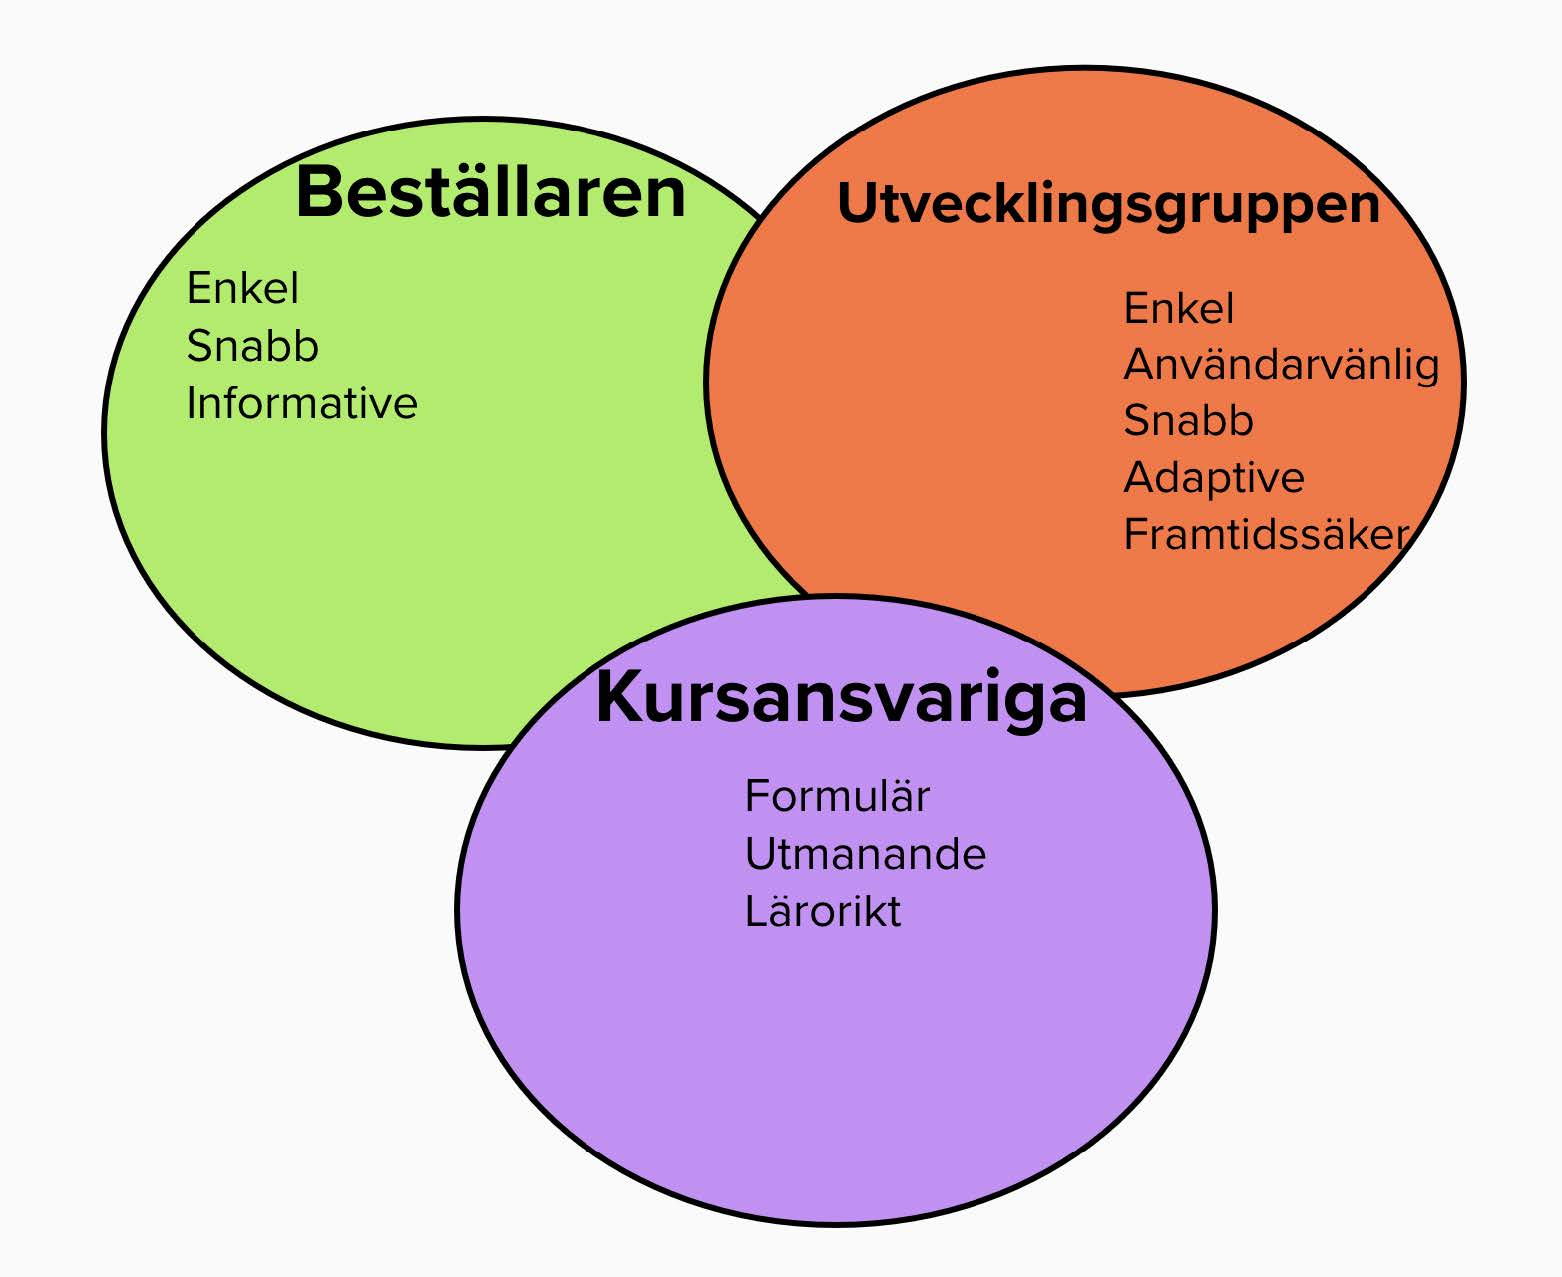
\includegraphics[width = 155px]{malbild.jpg}
    \caption{Målbild venndiagram}
    \label{fig:Målbild}
\end{figure}

Hur stabil är målbilden?

\begin{enumerate}
	\item Vårt digitala rapporteringsverktyg är inte helt nyskapande utan det finns liknande
lösningar som exempelvis Google Forms men vår lösning kommer med några unika
funktioner som är skräddarsydda med större kontroll över distribution och
administration. 

	 \item Helsingborg Convention and Event Bureau(HCEB) har erfarenhet av datainsamling
men saknar ett system som kan sammanställa datan. HCEB har således inte
mycket erfarenhet av själva mjukvaruutvecklingen. På grund av deras begränsade kunskap har vi friare händer att bestämma över produkten.

\item I Informationen vi fått från HCEB framgår inte mer än att beställaren vill ha en sammanställning av data som aktörer skickar in. På grund av den begränsade informationen kan vi anta att vi inte kan få en större mängd feedback på själva utvecklingen.

\item Eftersom HCEB är mer intresserade av att det finns ett färdigutvecklat system och
inte några specifika funktioner kommer troligtvis förändringar av utvecklingen att
välkomnas.

\item Kontakten hålls vid förutbestämda handledningstillfällen med jämna mellanrum och
vid behov kommer möten bokas för tydlighetens skull.

\item Tidigare har projektgruppen gjort en liknande utvecklingsprocess och har någorlunda
erfarenhet av utvecklingsarbetet och liknande tekniker.

\item Slutanvändarna har liknande intressen av arbetet och produkten som utvecklas.
\end{enumerate}


\newpage
\section{Process}
\subsection{Processmodell}

Projektgruppens analys av målbilden pekar mer mot en lättrörlig modell eftersom vi har begränsat med information och kunskap i början av projektet.
Det krävs att gruppen kan agera snabbare när det gäller att ta beslut om arbetet verkar gå åt fel håll, vilket är vanligt i början. Beslut kan tas i
efterhand om det exempelvis skulle dyka upp krav som vi inte tänkt på vilket gör
utvecklingen mer flexibel och anpassbar. En lättrörlig modell kommer ge projektgruppen
möjlighet att jobba med en testbar produkt under längs utvecklingens gång istället för endast
en slutprodukt. Senare i projektet kommer vi jobba mer med en iterativ process eftersom vi
då har vi fått en tydligare målbild och kan strukturera upp arbetet.
\subsection{WBS}
Då vi fortfarande befinner oss i början av projektet har vi begränsad information. Därför har vi valt att dela arbetet i breda kategorier. På nivå 1 i vår WBS ligger slutprodukten som har givits namnet Sustainable Form. De kategorier på nivå 2 är sådana som vi vet att vi kommer behöva göra: 
\begin{itemize}
\item Databas
\item Grafiskt användargränssnitt, GUI
\item Test
\item Design + Prototyp
\item API
\end{itemize}
\begin{figure}[htp]
    \centering
    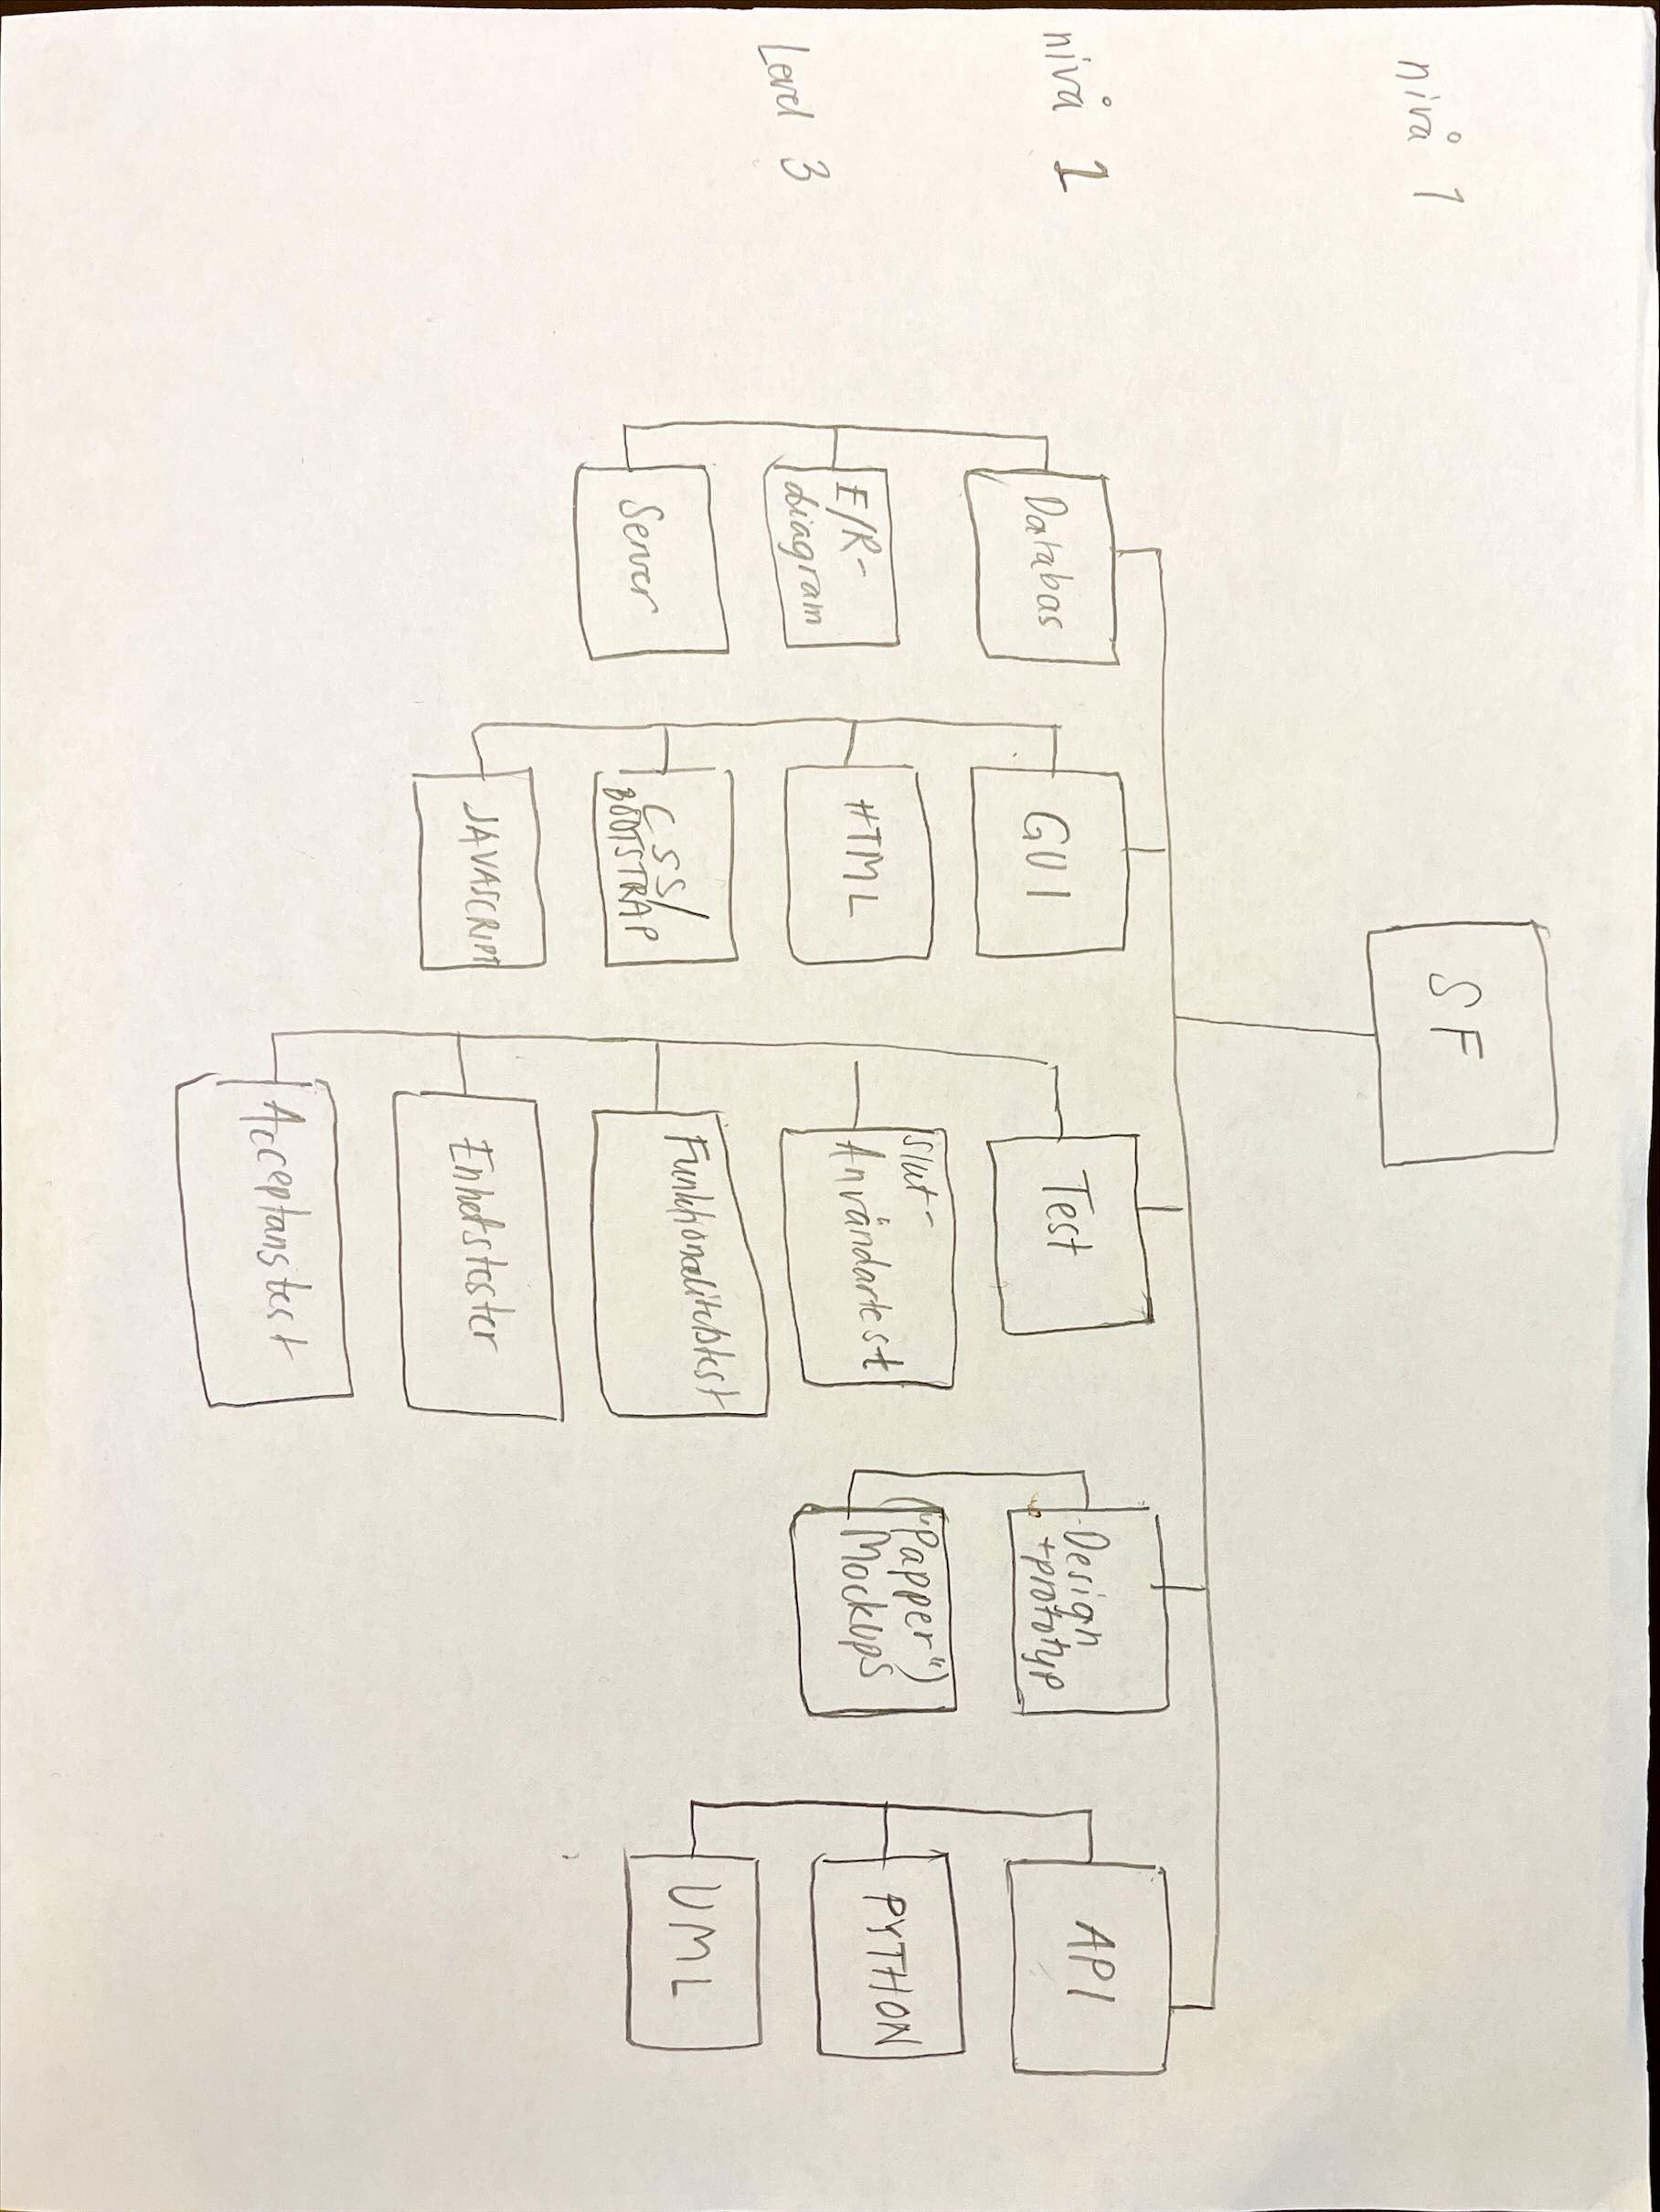
\includegraphics[width = 175px,angle=90]{WBS.jpg}
    \caption{WBS graf}
    \label{fig:WBS graf}
\end{figure}

Varje modul delades upp i underuppgifter som sattes in i WBS på nivå 3. Databasen består av arbetsuppgifterna E\&R-diagram och server, GUI:n består av HTML, CSS\&Bootstrap och JavaScript och under testmodulen hittar vi användartest, funktionstest, enhetstester och acceptanstest. Modulen Design\&Prototyp har en underuppgift "paper mockups", dvs att tillverka low fidelity-prototyper, och slutligen så har API som submoduler python och UML. Vi har valt att använda python eftersom ingen i teamet har gjort något projekt i python tidigare och det känns orimligt att ta examen från LTH och inte ha jobbat i det språket.
\subsection{PERT}

Det är lite svårt att veta var man ska börja eftersom vi inte har så mycket kunskap om projektet än. Vi tänkte att en design-mockup är ett bra ställe att börja på eftersom det kan involvera kunden tidigt. Dessutom hjälpte PERT oss att se sambanden mellan de olika aktiviteterna. Vi har tvingats att tänka på arbetsbördan på ett mycket konkret sätt. Det blir också tydligt att vissa aktiviteter tar betydligt längre tid än andra. \\
\\
\noindent
Om vi skulle hamna i tidsnöd och inte ha tid att implementera alla krav så skulle vi prioritera de krav som har med insamlande av data att göra. Dessutom skulle krav som har tillkommit - att Miljöförvaltningen ska få ställa några frågor extra frågor - få strykas. \\
\\
\noindent
Enligt kursbeskrivningen förväntas vi lägga 96 timmar på självstudier under lp3. Vi har alltså resurser på 576 timmar i projektgruppen. Om vi räknar ihop timmarna i kolumnen "mellan" nedan så blir det 523 timmar. Då har vi råd med att någonting tar längre tid. Förhoppningsvis blir det även någon modul som tar mindre tid än beräknat.
\\
\\
\\
\begin{tabular}{c||c||c||c}
    ID & är beroende av... & Beskrivning av aktivitet/mål & Tidsuppskattning \\
   \hline
    &&& \begin{tabular}{ccc}
         Låg & Mellan & Hög  \\
 
    \end{tabular}
  \\
\hline
  1 & - & Design mockup & \begin{tabular}{ccc}
                            6 h & 12 h & 18 h \\
      
      
                            \end{tabular}
  \\
  \hline
  2 & - & E/R-diagram & \begin{tabular}{ccc}
                         2 h & 3 h & 4 h  \\
       
                        \end{tabular}
  \\
  \hline
    3 & - & GUI & \begin{tabular}{ccc}
                         30 h & 48 h & 60 h  \\
       
                        \end{tabular}
  \\
    \hline
    4 & Databasen och GUI & API & \begin{tabular}{ccc}
                         120 h & 240 h & 480 h  \\
       
                        \end{tabular}
  \\
  
    \hline
    5 & E/R-diagram & Databas & \begin{tabular}{ccc}
                        10 h  & 16 h & 24 h  \\
       
                        \end{tabular}
  \\
  
    \hline
    6 & - & JavaScript & \begin{tabular}{ccc}
                        8 h & 16 h &  24 h \\
       
                        \end{tabular}
  \\
    \hline
    7 & - & UML & \begin{tabular}{ccc}
                         8h & 12 h & 16 h  \\
       
                        \end{tabular}
  \\
    \hline
    8 & - & Användartest & \begin{tabular}{ccc}
                         4 h & 8 h & 12 h  \\
       
                        \end{tabular}
  \\
    \hline
    9 & - & Funktionstest & \begin{tabular}{ccc}
                         60 h & 120 h & 240 h  \\
       
                        \end{tabular}
  \\
    \hline
    10 & - & Databastest & \begin{tabular}{ccc}
                         24 h & 48 h & 92 h  \\
       
                        \end{tabular}
  \\
  
\end{tabular}

\newpage
\begin{figure}[htp]
    \centering
    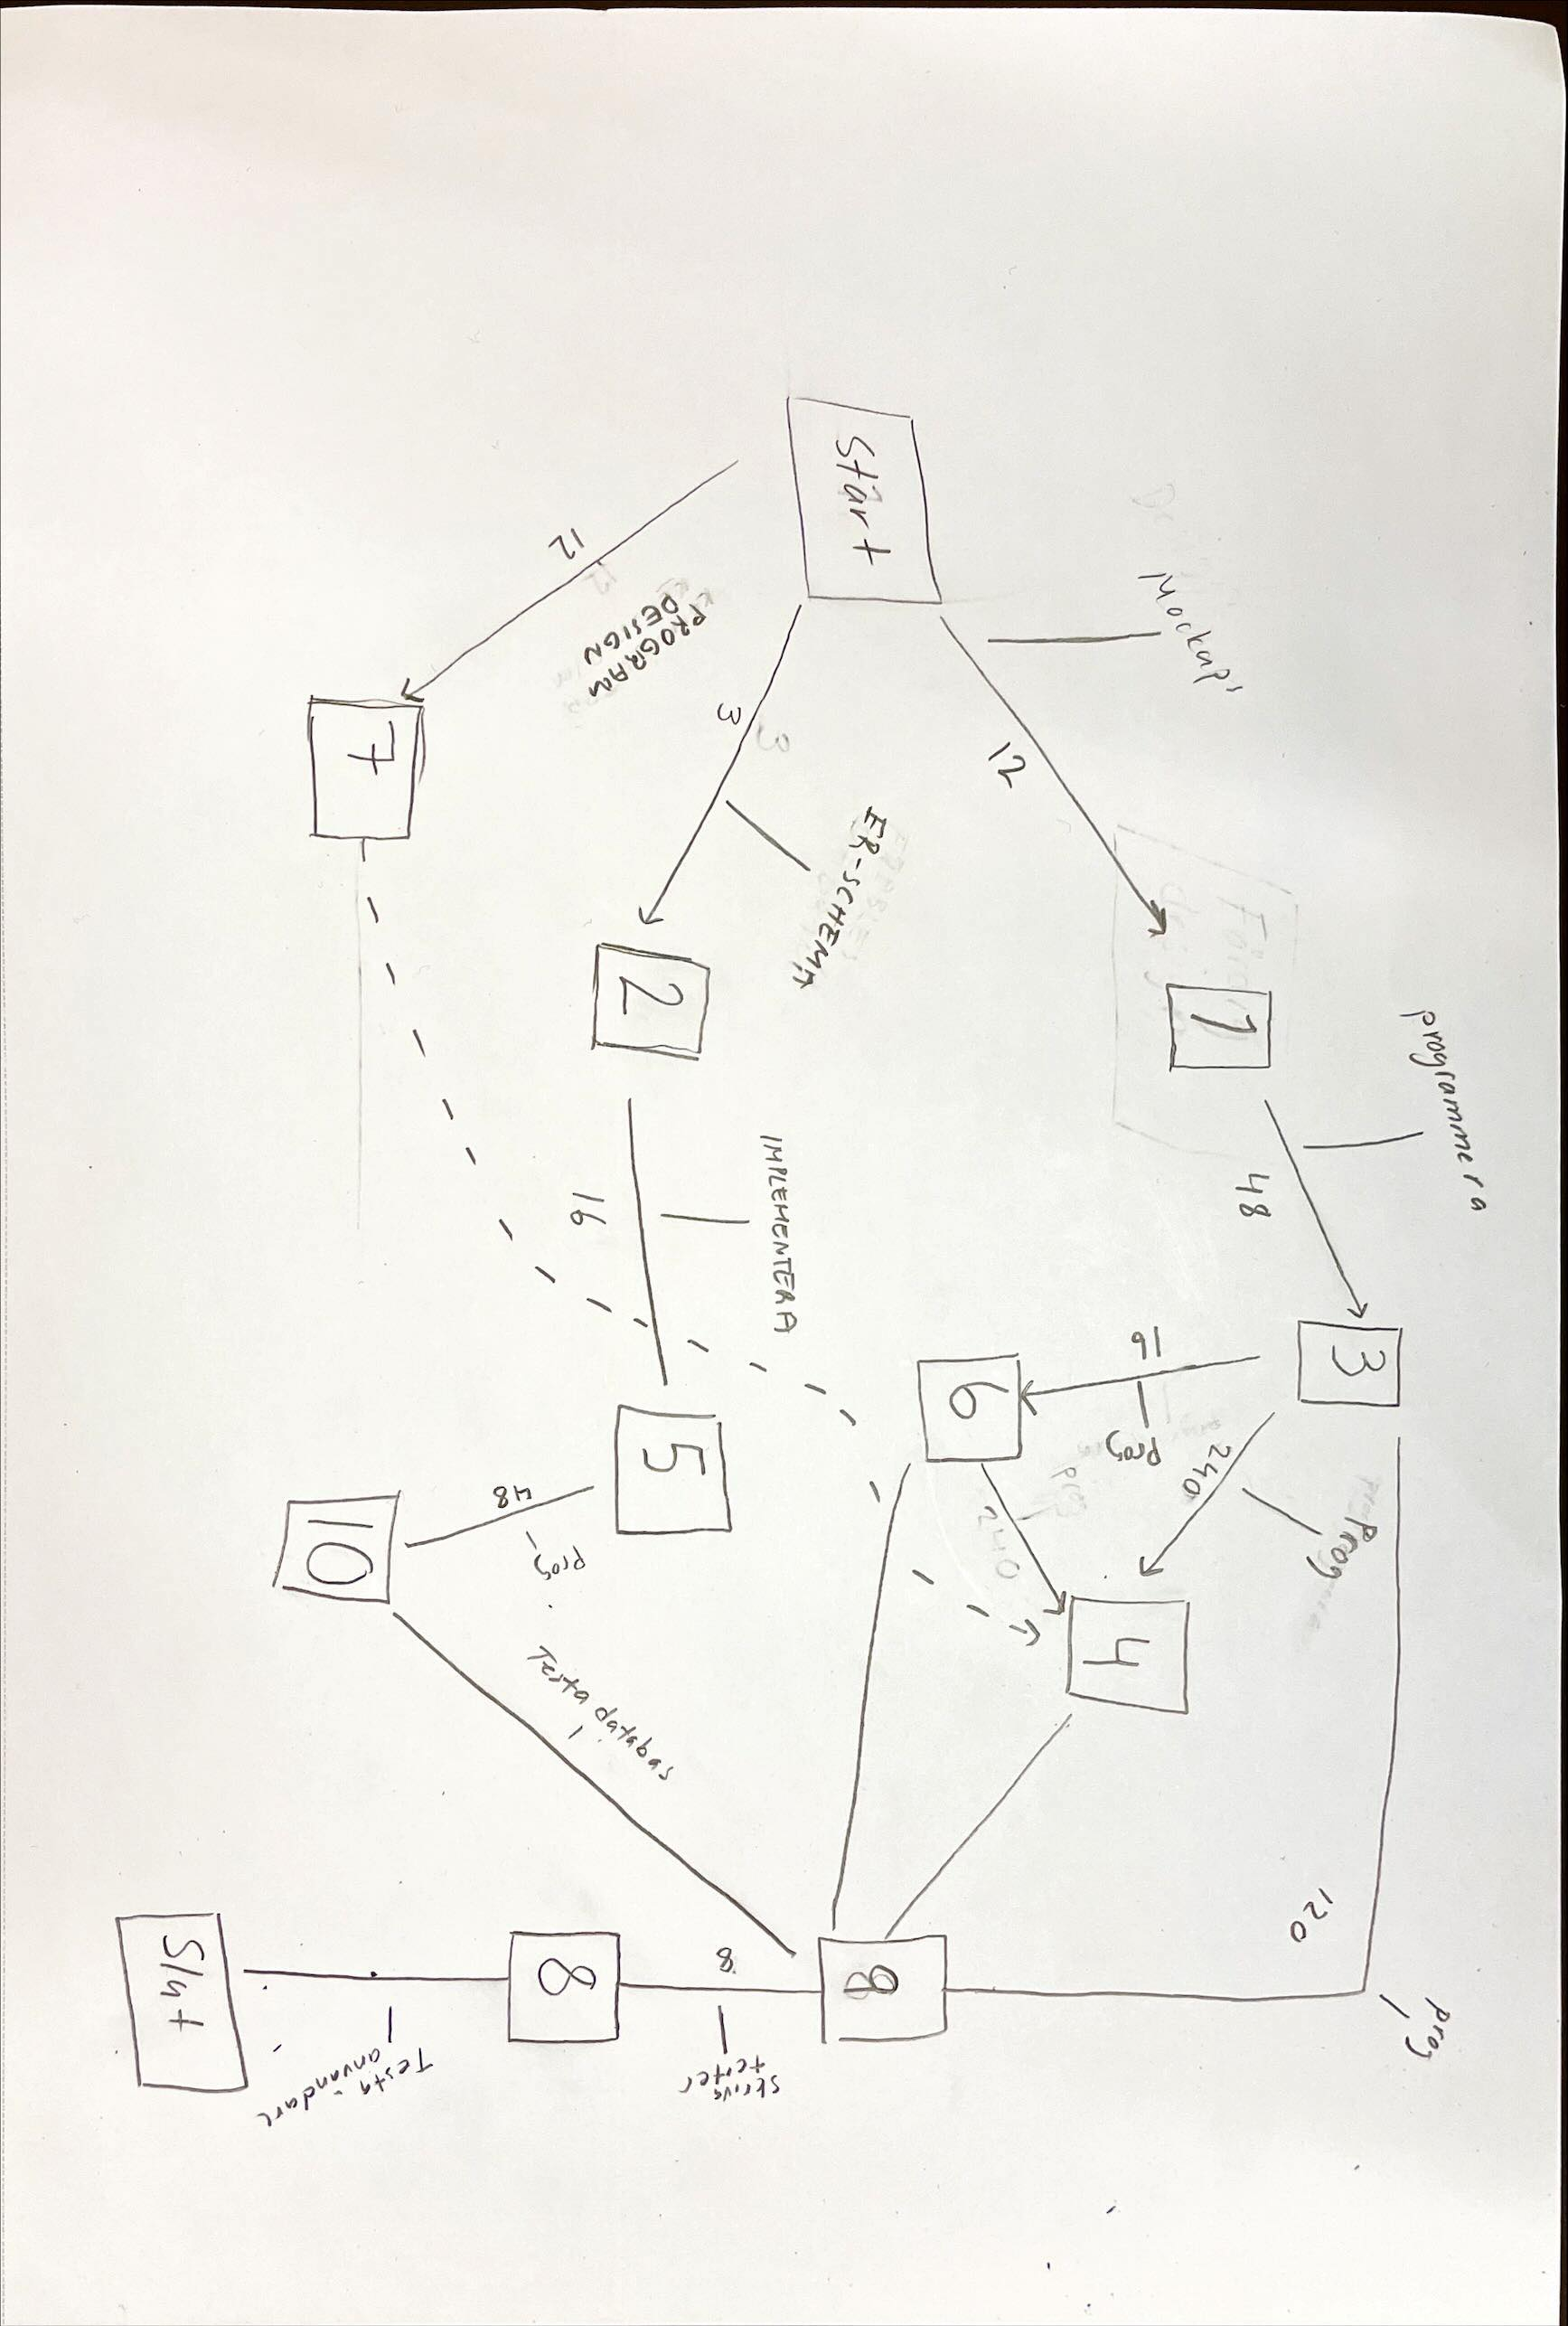
\includegraphics[width = 165px, angle=90]{Pert.jpg}
    \caption{PERT graf}
    \label{fig:PERT graf}
\end{figure}


\subsection{Tidsplan}

\begin{figure}[htp]
    \centering
    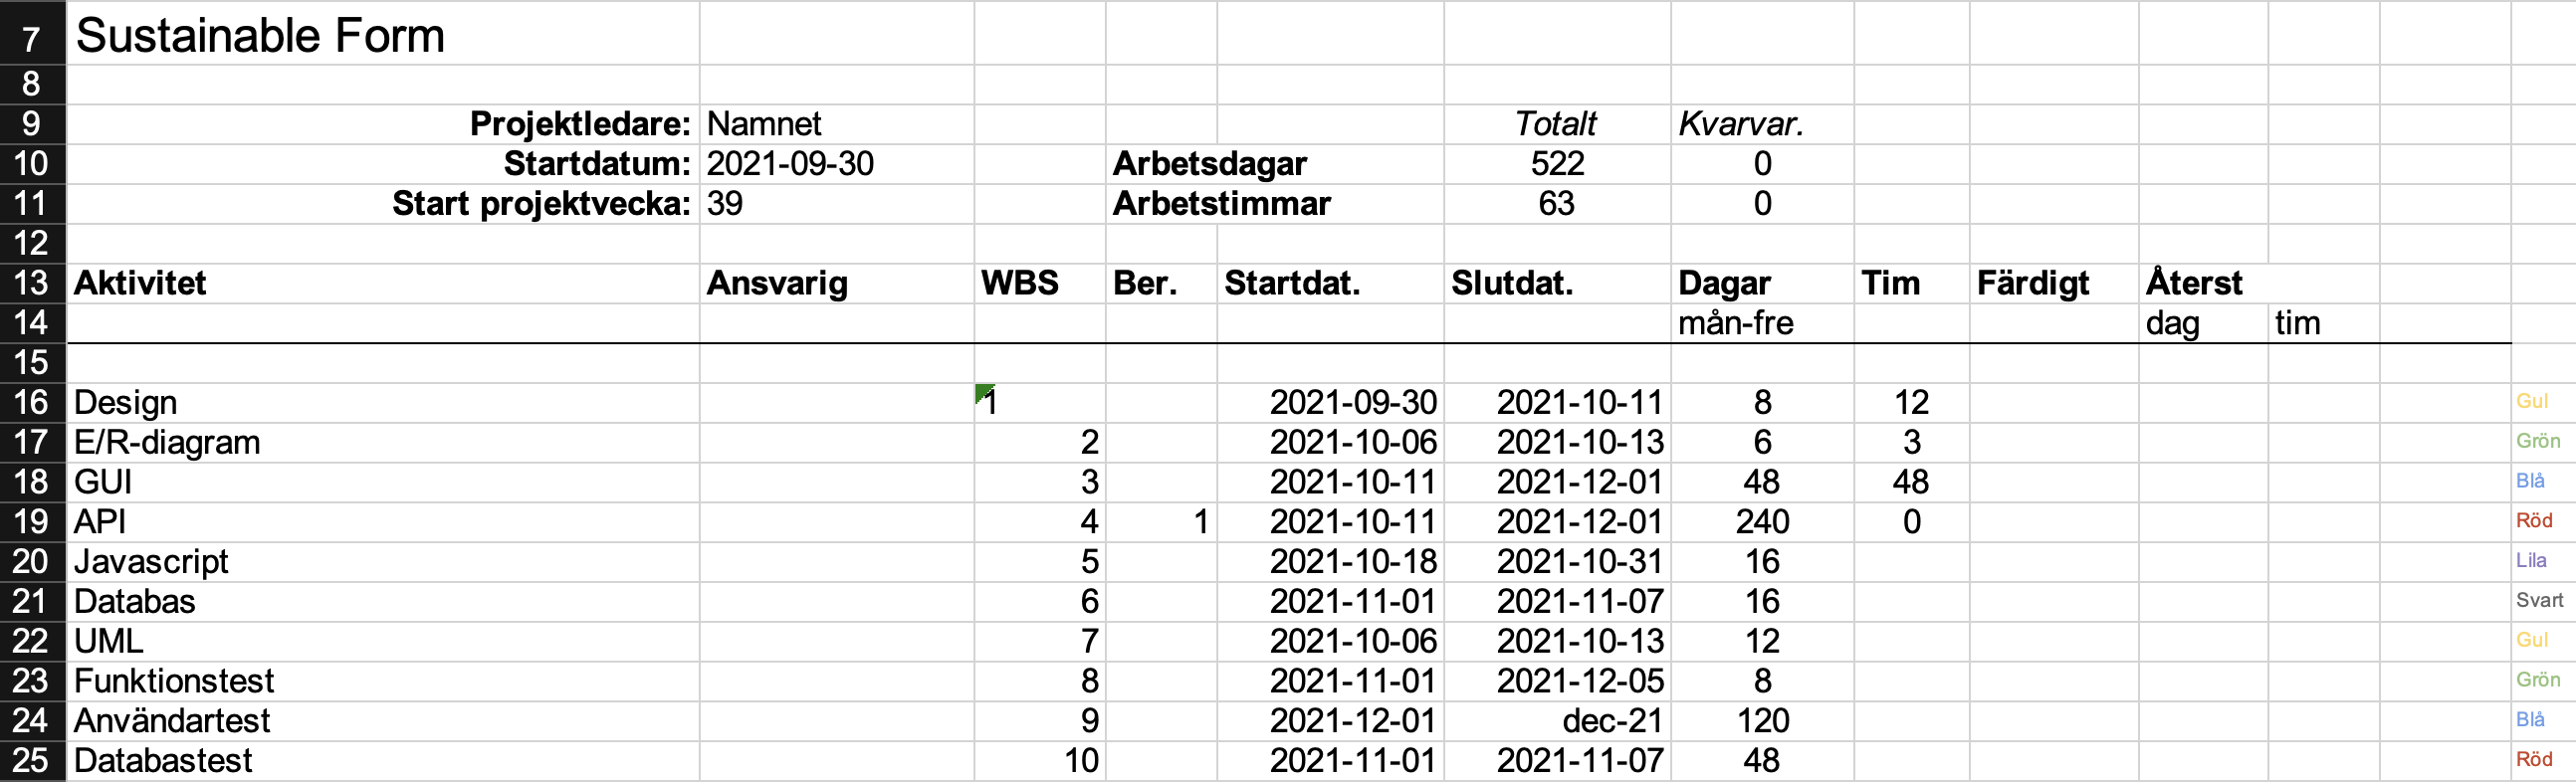
\includegraphics[width = 450px]{gantt1.png}
    \caption{Gant tidsplan}
    \label{fig:Gant tidsplan}
\end{figure}

\begin{figure}[htp]
    \centering
    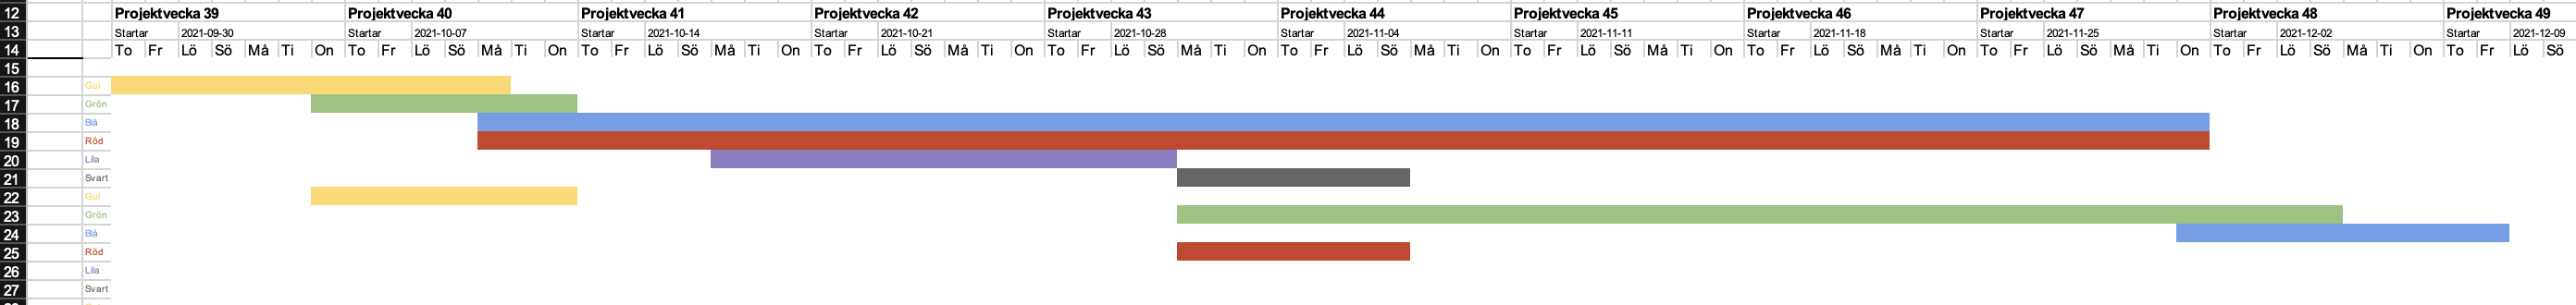
\includegraphics[width = 450px]{Gantt2.png}
    \caption{Gant tidsplans schema}
    \label{fig:Gant tidsplans schema}
\end{figure}
\newpage
\section{Team}

En diskussion som gruppen har fört är hur vi kan förebygga "the five dysfunctions" som Günther pratade om under sin föreläsning. Vi har
kommit fram till att "absence of trust" kan förebyggas genom att bli bättre på att kommunicera med varandra. Vi är ju alla vuxna och ska kunna ta en diskussion. Vad det gäller "fear of conflict" har vi
bestämt att man ska kunna kräva en debatt för att reda ut saker som känns oklart. Det kan ibland
vara svårt att veta vilken roll man har och det skulle underlätta om det fanns tydliga
rollfördelningar då detta skulle ge en klarare uppfattning om vilka ansvarsområden som finns. Om någon inte vet vad de ska
göra kan det leda till passivitet. Det kan i sin tur skapa konflikter eftersom passitivitet lätt bidrar till osäkerhet. Det kan vara bra att ha ground rules som hjälp för att undvika hamna i en
sådan situation. \\
Med rollfördelningen och fördelning av ansvar kan vi förebygga "lack of
commitment". På så sätt vet gruppen bättre vad som förväntas av dem och vad deras ansvarsområde kräver. Det kommer bidra till att missförstånd förhoppningsvis undviks och att
varje gruppmedlem kan vara engagerad och hängiven projektarbetet. Även här kan det vara bra
att ta hjälp av ground rules. För "Avoidance of Accountability" kan Scrumboarden hjälpa oss att
konkret se vilken gruppmedlem som har tagit sig an en viss uppgift. Det är viktigt att diskutera
varför olika uppgifter behöver göras för att säkerställa att alla förstår och är överens om vad
gruppen arbetar mot.


\subsection{Ground Rules}

\subsubsection{Arbetsformer}

Vi ska utnyttja delgrupperna och arbeta främst inom dessa. Om vi sitter fast med något tar
vi i första hand hjälp av de andra i delgruppen. Arbetsuppgifterna jobbar vi med utifrån
scrumboarden. Den uppgift som står högst upp på scrumboarden ska bli tagen först. När man har tagit en uppgift har man fullt ansvar för
att den slutförs. Gruppen jobbar både på distans men även på plats i campus. Under en
vecka har vi två möten, det ena på måndagar som är på plats i skolan och det andra mötet är
online på fredagar. Feedback från gruppen fås på fredagsmöten där vi har en genomgång av
vad den enskilde gruppmedlemmen har jobbat med under veckan.

\subsubsection{Kontaktinfo}

För att säkerställa att alla gruppmedlemmar har fått rätt information har vi kommunikation på
discord. Det är ens egna ansvar att reagera på de inläggen som görs som en indikation på att
alla har tagit del av informationen. Vi har även många möten som diskuterat tidigare och det
kommer möjliggöra även mer att vi får rätt information i tid. Det är uppmanad inom gruppen
att kolla på discord några gånger dagligen mellan kl 08.00-16.00.

\subsubsection{Projektmöten}

Gruppmöten är professionella och syftar till att bidra med projektets utveckling och därför
ska man i förväg meddela ifall man har fått förhinder och inte kan medverka på ett möte. Alla
ska lyssna på det som övriga deltagare tar upp och aktiv delta i diskussionen.
Mötesanteckningar tas under mötet och överförs till dagordningen som ska vara tillgängliga
för alla gruppmedlemmar.

\subsection{Ansvarsområden}
Det här stycket redogör för vilka ansvarsområden vi har identifierat och vilka egenskaper som passar för dessa. Många av egenskaperna ska självklart finnas hos hela projektgruppen men vi tyckte ändå att det var värt att ha med dem explicit.

\subsubsection{Kravprocessboken}
\begin{itemize}
\item Insatt i kravarbetet
\item Ha en övergripande kunskap om projektet
\item Noggrann
\item Vara kunnig i LaTex
\end{itemize}

\subsubsection{Processboken}
\begin{itemize}
\item Vara mycket väl insatt i övningarna
\item Ha en övergripande kunskap i projektet
\item Noggrann
\item Vara kunnig i LaTex
\end{itemize}

\subsubsection{Kravdokumentet}
\begin{itemize}
\item Mycket kunnig i hur krav formuleras
\item Detaljkunnig
\item Kunnig i semantik och språk
\item Väl insatt i rapporteringsverktygets funktioner
\end{itemize}

\subsubsection{Scrumboarden}
\begin{itemize}
\item Administrativ
\item Ha en övergripande koll på alla uppgifter som ska göras i projektet - särskilt de som ska med i nästa sprint
\item Strukturerad
\item Ordningsam
\end{itemize}

\subsubsection{Mailkontakt med beställare}
\begin{itemize}
\item Ha god social förmåga
\item Bra på att kommunicera i skrift
\item Uppdaterad
\item Administrativ
\end{itemize}

\subsubsection{Hålla i möten}
\begin{itemize}
\item Vara bekväm i ledarroll
\item Strukturerad
\item Förmåga att kunna fokusera på det som är relevant
\end{itemize}

\subsection{Förväntningar}

De ansvariga för något av ovanstående områden förväntas ha många av egenskaperna för att
leva upp till de förväntningar som ställs för projektets bästa och utveckling framåt. Det ställs i
stort sätt samma krav på alla ansvarsområden. Att man är kommunikativ och aktiv samt delar
med sig av nyheter eller ändringar inom respektive ansvarsområde. Detta för att alla ska ha en
möjlighet att ta del av informationen och vara uppdaterade. Mer noggrannare innebär det att
den som är ansvarig för processboken har deltagit på möten och workshops. För
kravdokument krävs det att den ansvarige har koll på produkten och vet hur den ska fungera
dvs har en helhetsperspektiv om projektet. Ansvariga för scrum boarden måste vara
uppdaterad kring projektet och har övergripande koll på det aktuella arbetet. Stort ansvar
ligger hos personen som har hand om mail att denne är responsiv och når ut med viktig
information till andra inom gruppen. Det är ytterst viktigt att de ansvariga för
möten/dagordning vet om vad som är relevant i dagsläget att ta upp på möten för att de ska
vara effektiva.

\subsection{Belbin-test}

Eftersom människor har olika styrkor och svagheter ger det oss vissa särskilda beteenden.
Kunskap från Belbin-testet kan göra det enklare att dela ut roller eftersom det ger en inblick i
hur varje person fungerar. Medlemmar i gruppen får en bättre förståelse över hur personer i
gruppen fungerar i vissa situationer och kan lättare komma fram till bra lösningar som passar
alla. I projektgruppen kan det till exempel handla om att under övningar bättre kunna få fram
medlemmarnas tankar och funderingar. Detta kan hjälpa om man sedan tidigare vet om att en
viss person tenderar att inte föra fram sin åsikt kan man istället ställa fler frågor till denne. Ett
annat fall kan vara om projektledaren har en vana av att vara av en perfektionist och vill att
allt ska lösas på dennes villkor och önskan. Det kan bli betydligt svårare för projektledaren att
delegera ut arbete inom gruppen och då kan det vara fördelaktigt att andra gruppmedlemmar
kan våga säga ifrån och erbjuda hjälp.
\section{Resultat/ Risker}

\subsection{Brainstorma risker av olika slag}
\subsubsection{Projektrisker}
Risker som påverkar tidsplanen eller andra resursaspekter. 
\begin{enumerate}
\item Dålig kommunikation och missförstånd.
\item Dålig uppskattning av tid.
\item Förändringar i kraven.
\item Oförutsätbara händelser som till exempel sjukdom.
\item Konflikter inom gruppen.
\item Dålig struktur/planering av projektet.
\item Kompetens saknas (till exempel kunskaper i Python).
\item Brist på erfarenhet.
\item Vi får inte tillgång till hur utdata från vårt system ska formateras i tid.
\item Upptagen kontaktperson vilket kan resultera i långsamma svar.
\end{enumerate}

\subsubsection{Produktrisker}
Risker som påverkar prestandan eller kvaliteten på produkten.
\begin{enumerate}
    \item Vi uppfyller inte kraven.
    \item Produkten är inte tillräckligt intuitiv och enkel att använda med tanke på att användarna har så olika kunskaper och erfarenhet.
    \item Dåligt utformad kod - svårt att lägga till och ändra funktioner.
    \item Bristande javadokumentatiom.
    \item För lite testning som kan leda till bristande kvalitet.
    \item För få fyller i formuläret.
    \item För dålig servertjänst som kan leder till bland annat överbelastning.
    \item Vi lyckas inte deploya produkten - exempelvis problem med servern som vi inte kan förutse nu.
    \item Produkten är inte tillräckligt säker.
    \item Dåliga tester som förvränger värdefull data.
\end{enumerate}

\subsubsection{Affärsrisker}
Risker som påverkar organisationen, förlorade intäkter.

\begin{enumerate}
    \item Systemet kommer inte till användning.
    \item Finns redan bättre verktyg som kunden väljer istället.
\end{enumerate}

\subsection{Riskanalys enligt miniriskmetoden}
Vi har här använt oss av en metod som kallas miniriskmetoden för att identifiera och analysera risker. Vi tog hjälp av "Riskanalys"[4] för att genomföra denna metoden. Det slutade med att vi har kommit fram till ett antal risker och ska nu uppskatta sannolikheten att det sker och konsekvensen att de sker på en skala 1-4. 
\\

\begin{center}
    \begin{tabular}{|c|c|c|c|c|}
      \hline
      \thead{\makecell{Risk-\\nummer}} & \thead{Projektrisk} & \thead{Sannolikhet} & \thead{Konsekvens} & \thead{Riskmått}\\
      \hline
      2 &\makecell{Dålig uppfattning \\ av tid} & 4 & 4 & 16 \\
      \hline
      5 &\makecell{Konflikter inom \\ gruppen} & 4 & 3 & 12 \\
      \hline
      1 &\makecell{Dålig kommunikation\\ och missförstånd} & 3 & 3 & 9 \\
      \hline
      6 &\makecell{Dålig planering av\\ projektet} & 4 & 2 & 8 \\
      \hline
      9 &\makecell{Försenad information \\ om format på utdata} & 4 & 2 & 8 \\
      \hline
     4 & \makecell{Oförutsägbara händelser} & 2 & 3 & 6 \\
      \hline
      8 & \makecell{Brist på erfarenhet} & 3 & 2 & 6 \\
      \hline
     10 & \makecell{Upptagen kontaktperson,\\innebär långsamma svar} & 2 & 3 & 6 \\
      \hline
     7 & \makecell{Kompetens saknas} & 4 & 1 & 4 \\
      \hline
     3 & \makecell{Förändringar\\i kraven} & 4 & 1 & 4 \\
      \hline
      \end{tabular}
\end{center}
      
      \begin{center}
    \begin{tabular}{|c|c|c|c|c|}
      \hline
      \thead{\makecell{Risk-\\nummer}} & \thead{Produktrisk} & \thead{Sannolikhet} & \thead{Konsekvens} & \thead{Riskmått}\\
       \hline
      2 & \makecell{Produkten är ej \\ tillräckligt intuitiv} & 2 & 4 & 8 \\
      \hline
     4 & \makecell{Bristande javadokumentation} & 4 & 2 & 8 \\
      \hline
      6 & \makecell{För få slutanvändare fyller\\ i formuläret} & 3 & 2 & 6 \\
      \hline
      5 & \makecell{För lite testning} & 3 & 2 & 6 \\
      \hline
      8 &\makecell{Lyckas ej implementera \\ hemsida på server} & 1 & 4 & 4 \\
      \hline
     7 & \makecell{dåligt val av servertjänst, \\leder till text\\överbelastning } & 1 & 4 & 4 \\
      \hline
     1 & \makecell{Uppfyller ej kraven} & 2 & 2 & 4 \\
      \hline
      9 &\makecell{Produkten är inte \\ tillräckligt säker} & 2 & 2 & 4 \\
      \hline
     3 &\makecell{Dåligt utformad kod} & 3 & 1 & 3 \\
      \hline
     10 & \makecell{Dåliga tester som \\förvränger värdefull\\data} & 1 & 1 & 1 \\
      \hline
    \end{tabular}
\end{center}

\newpage
\subsection{Utvärdering av risker enligt miniriskmetoden}
Här hart vi valt de tre av de rikser med högst riskmått från projket- och produktrisker. Vi har sedan sett vad vi ska vidta för återgärd och vad det förväntade utfallet av återgärden blir. 

 \begin{center}
    \begin{tabular}{ | c | c | c | c |}
      \hline
      \thead{\makecell{Risk-\\nummer}} & \thead{Projektrisk} & \thead{Åtgärd} & \thead{Förväntat utfall} \\
      \hline
      1 & \makecell{Dålig kommunikation\\ och missförstånd} &  \makecell{Tydligt kommunikationsplan \\ samt uppsatta ground roules.}  & \makecell{Bättre stämning och \\ minskad risk för missförstånd.} \\
      \hline
      1 & \makecell{Dålig tidsuppfattning} &  \makecell{En god struktur samt \\ kontinuerlig uppföjning \\under sprints.}  & \makecell{Bättre stämning och \\ En bättre uppfattning om \\ projektet ligger i fas.} \\
      \hline
      1 & \makecell{Konflikter inom \\ gruppen} &  \makecell{Respektera varandra, \\ god kommunikartion och, \\ visa förtroende för andra.}  & \makecell{Alla kommer trivas bättre och \\ mer framgångsrikt projekt.} \\
      \hline
       &\makecell{\textbf{Produktrisk}\\} &   &  \\
      \hline
     1 & \makecell{Produkten är ej \\ tillräckligt intuitiv} & Mer användartest.  & \makecell{Bättre helhetsbil av användare} \\
      \hline
       1 &\makecell{Bristande \\ javadokumentation} &\makecell{ Använd javas guide för\\ dokumentation.} & \makecell{Koden blir mer återanvändbar och \\ projektmedlemmarna får en större \\ förståelse över koden.} \\
      \hline
      1 & \makecell{För lite testning} & \makecell{Se till att ha en plan över\\ hur ofta och vad man testar.} & \makecell{Med en plan över hur ofta och vad  \\ man tester eliminerar\\ man risken att ha för få tester.} \\
      \hline
    \end{tabular}
  \end{center}
  
  \subsection{Hur sker uppföljning av risker?}
I början av varje sprint ska risker kopplade till de delmoment som sprinten innehåller identifieras och diskuteras. Eftersom vi använder oss av sprinter som löper i en vecka, kommer vi att i mitten av veckan under ett möte följa upp om någon av gruppmedlemmarna har stött på ett hinder. Om en gruppmedlem har stött på problem under sprinten, ska det problemet analyseras och jämföra om någon av de risker vi har dokumenterat stämmer överens med problemet. Eftersom vi har åtgärder för de risker vi har dokumenterat kan vi enklare hantera problemet, eftersom vi då har en tydlig riskhantering.


\section{Utveckling och process}


\section{Referenser}

\section{Bilagor}
\subsection{Arbetsblad från motivering och process workshop}


\begin{figure}[htp]
    \centering
    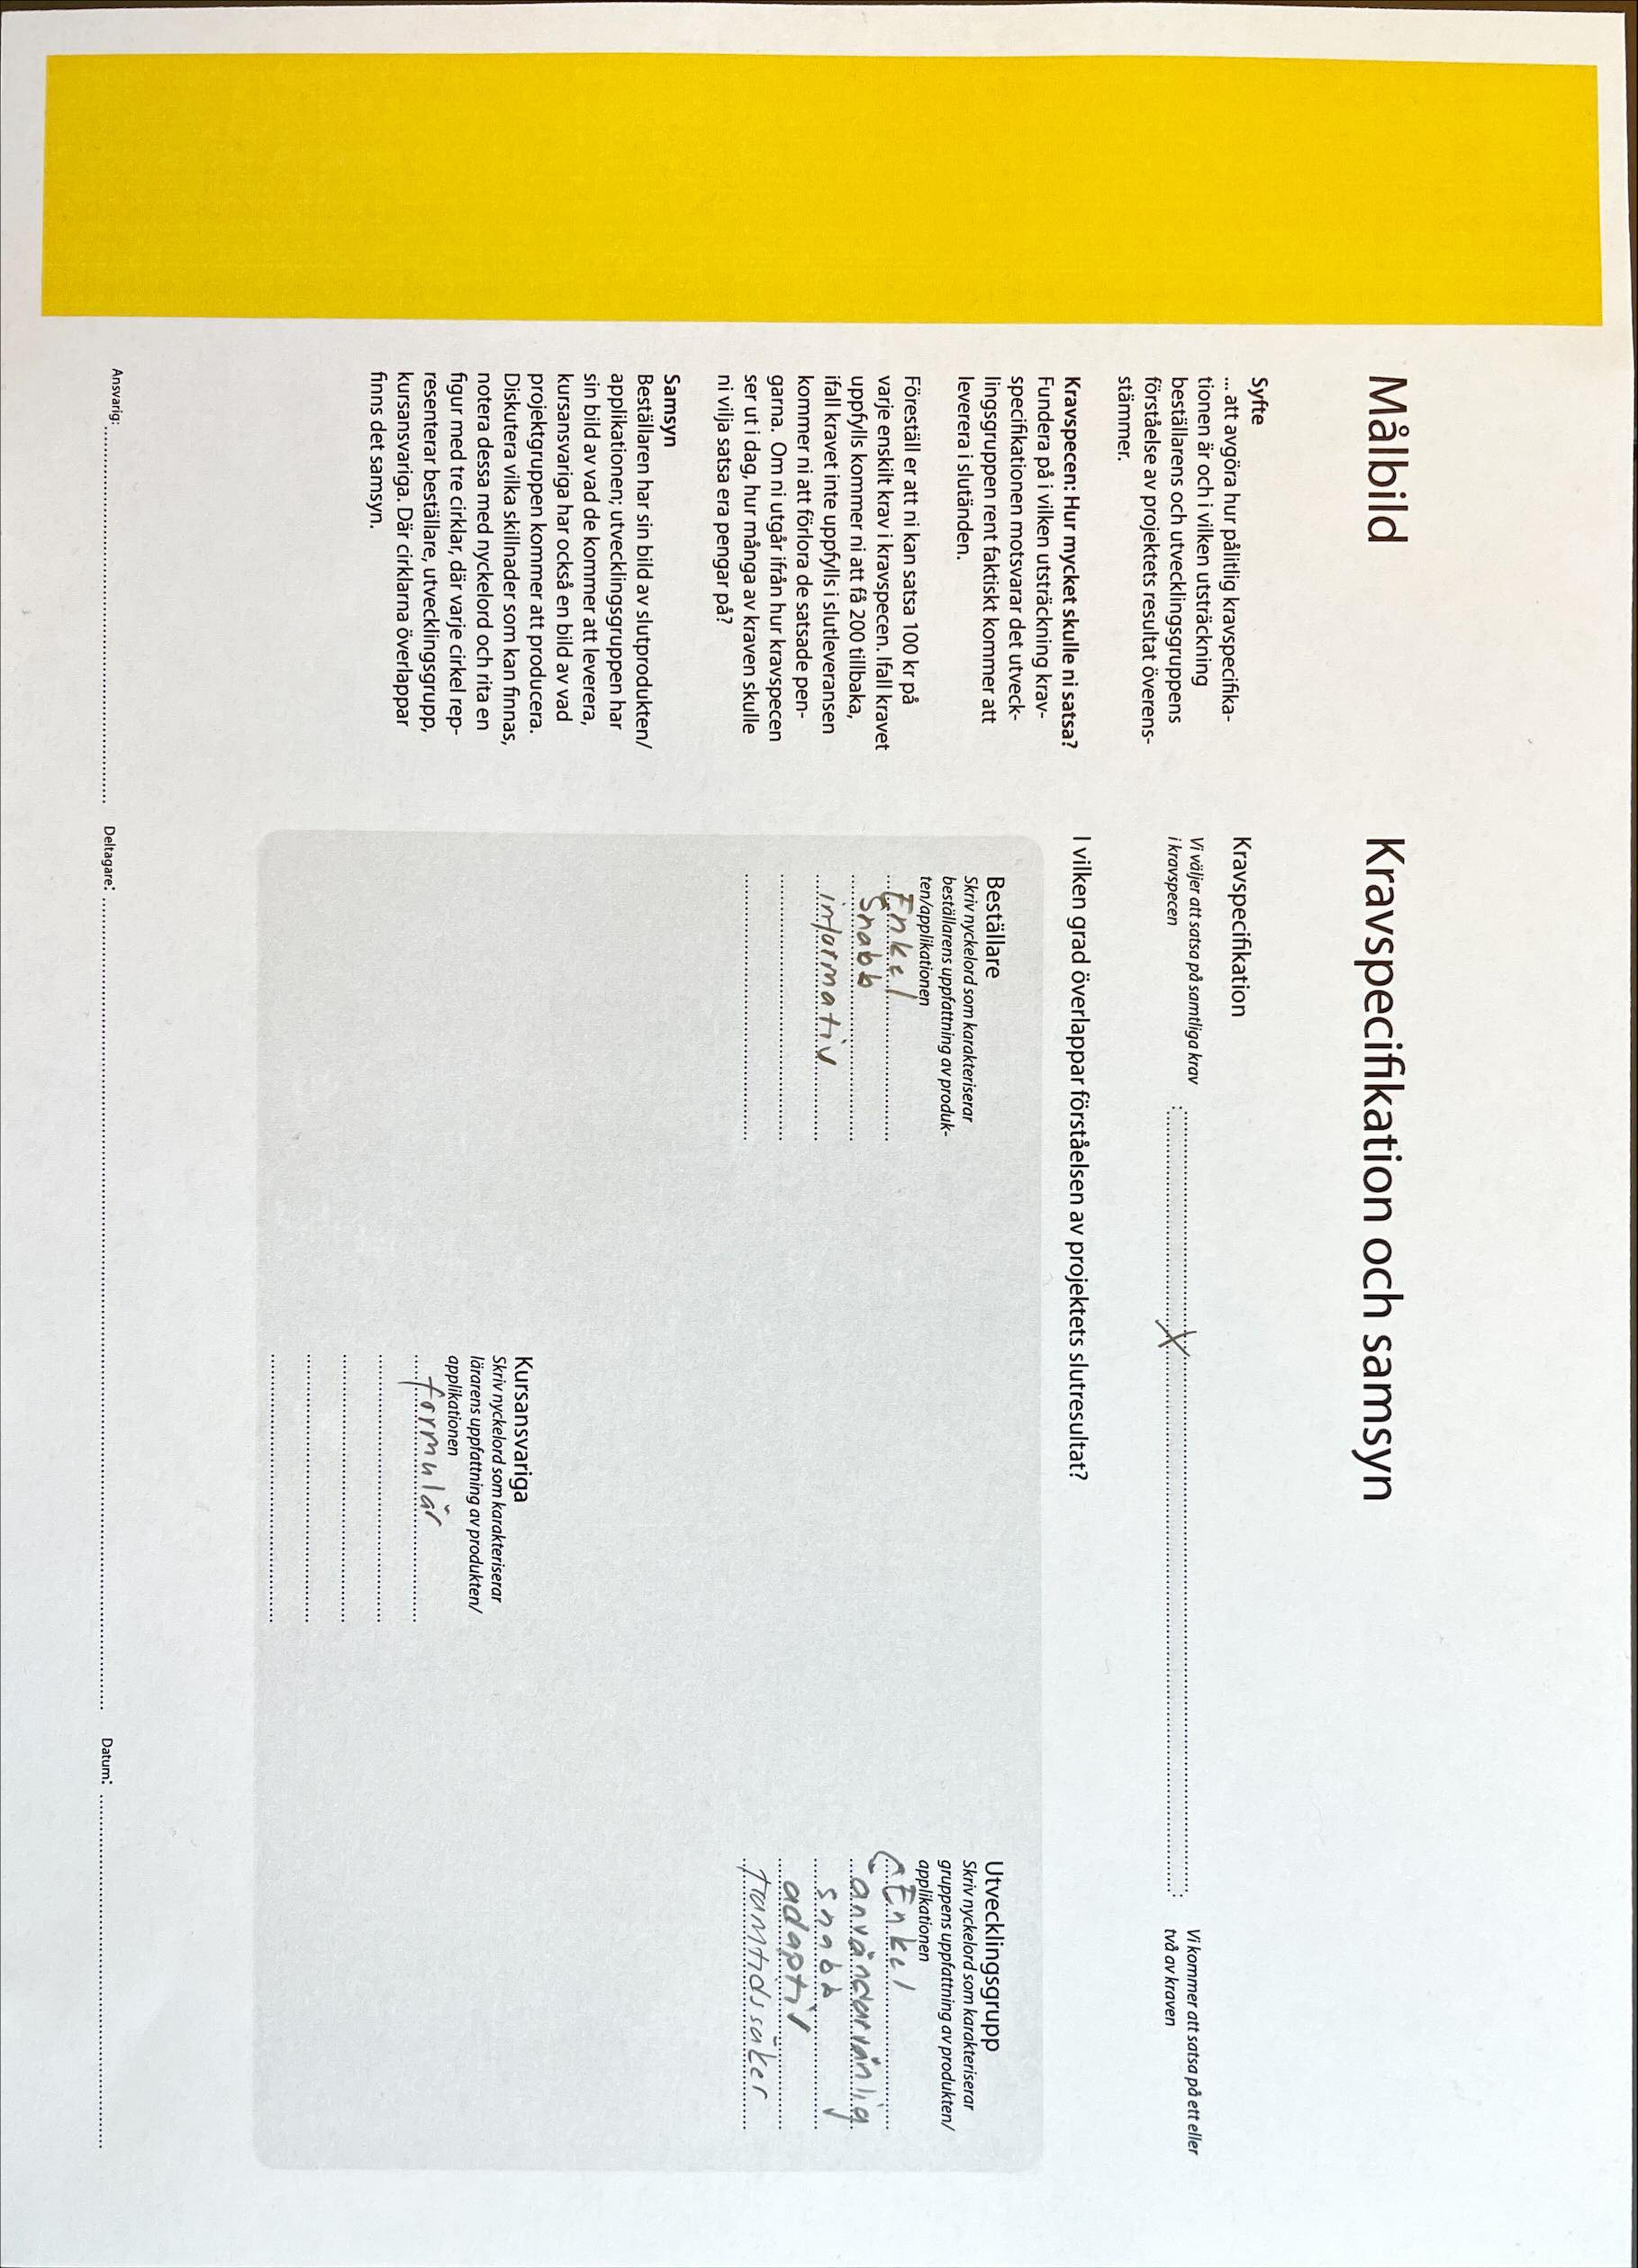
\includegraphics[width = 175px,angle=90]{KS.jpg}
    \caption{Arbetsblad från workshop. Kravspecification och samsyn}
    \label{fig:Bilaga samsyn}
\end{figure}

\begin{figure}[htp]
    \centering
    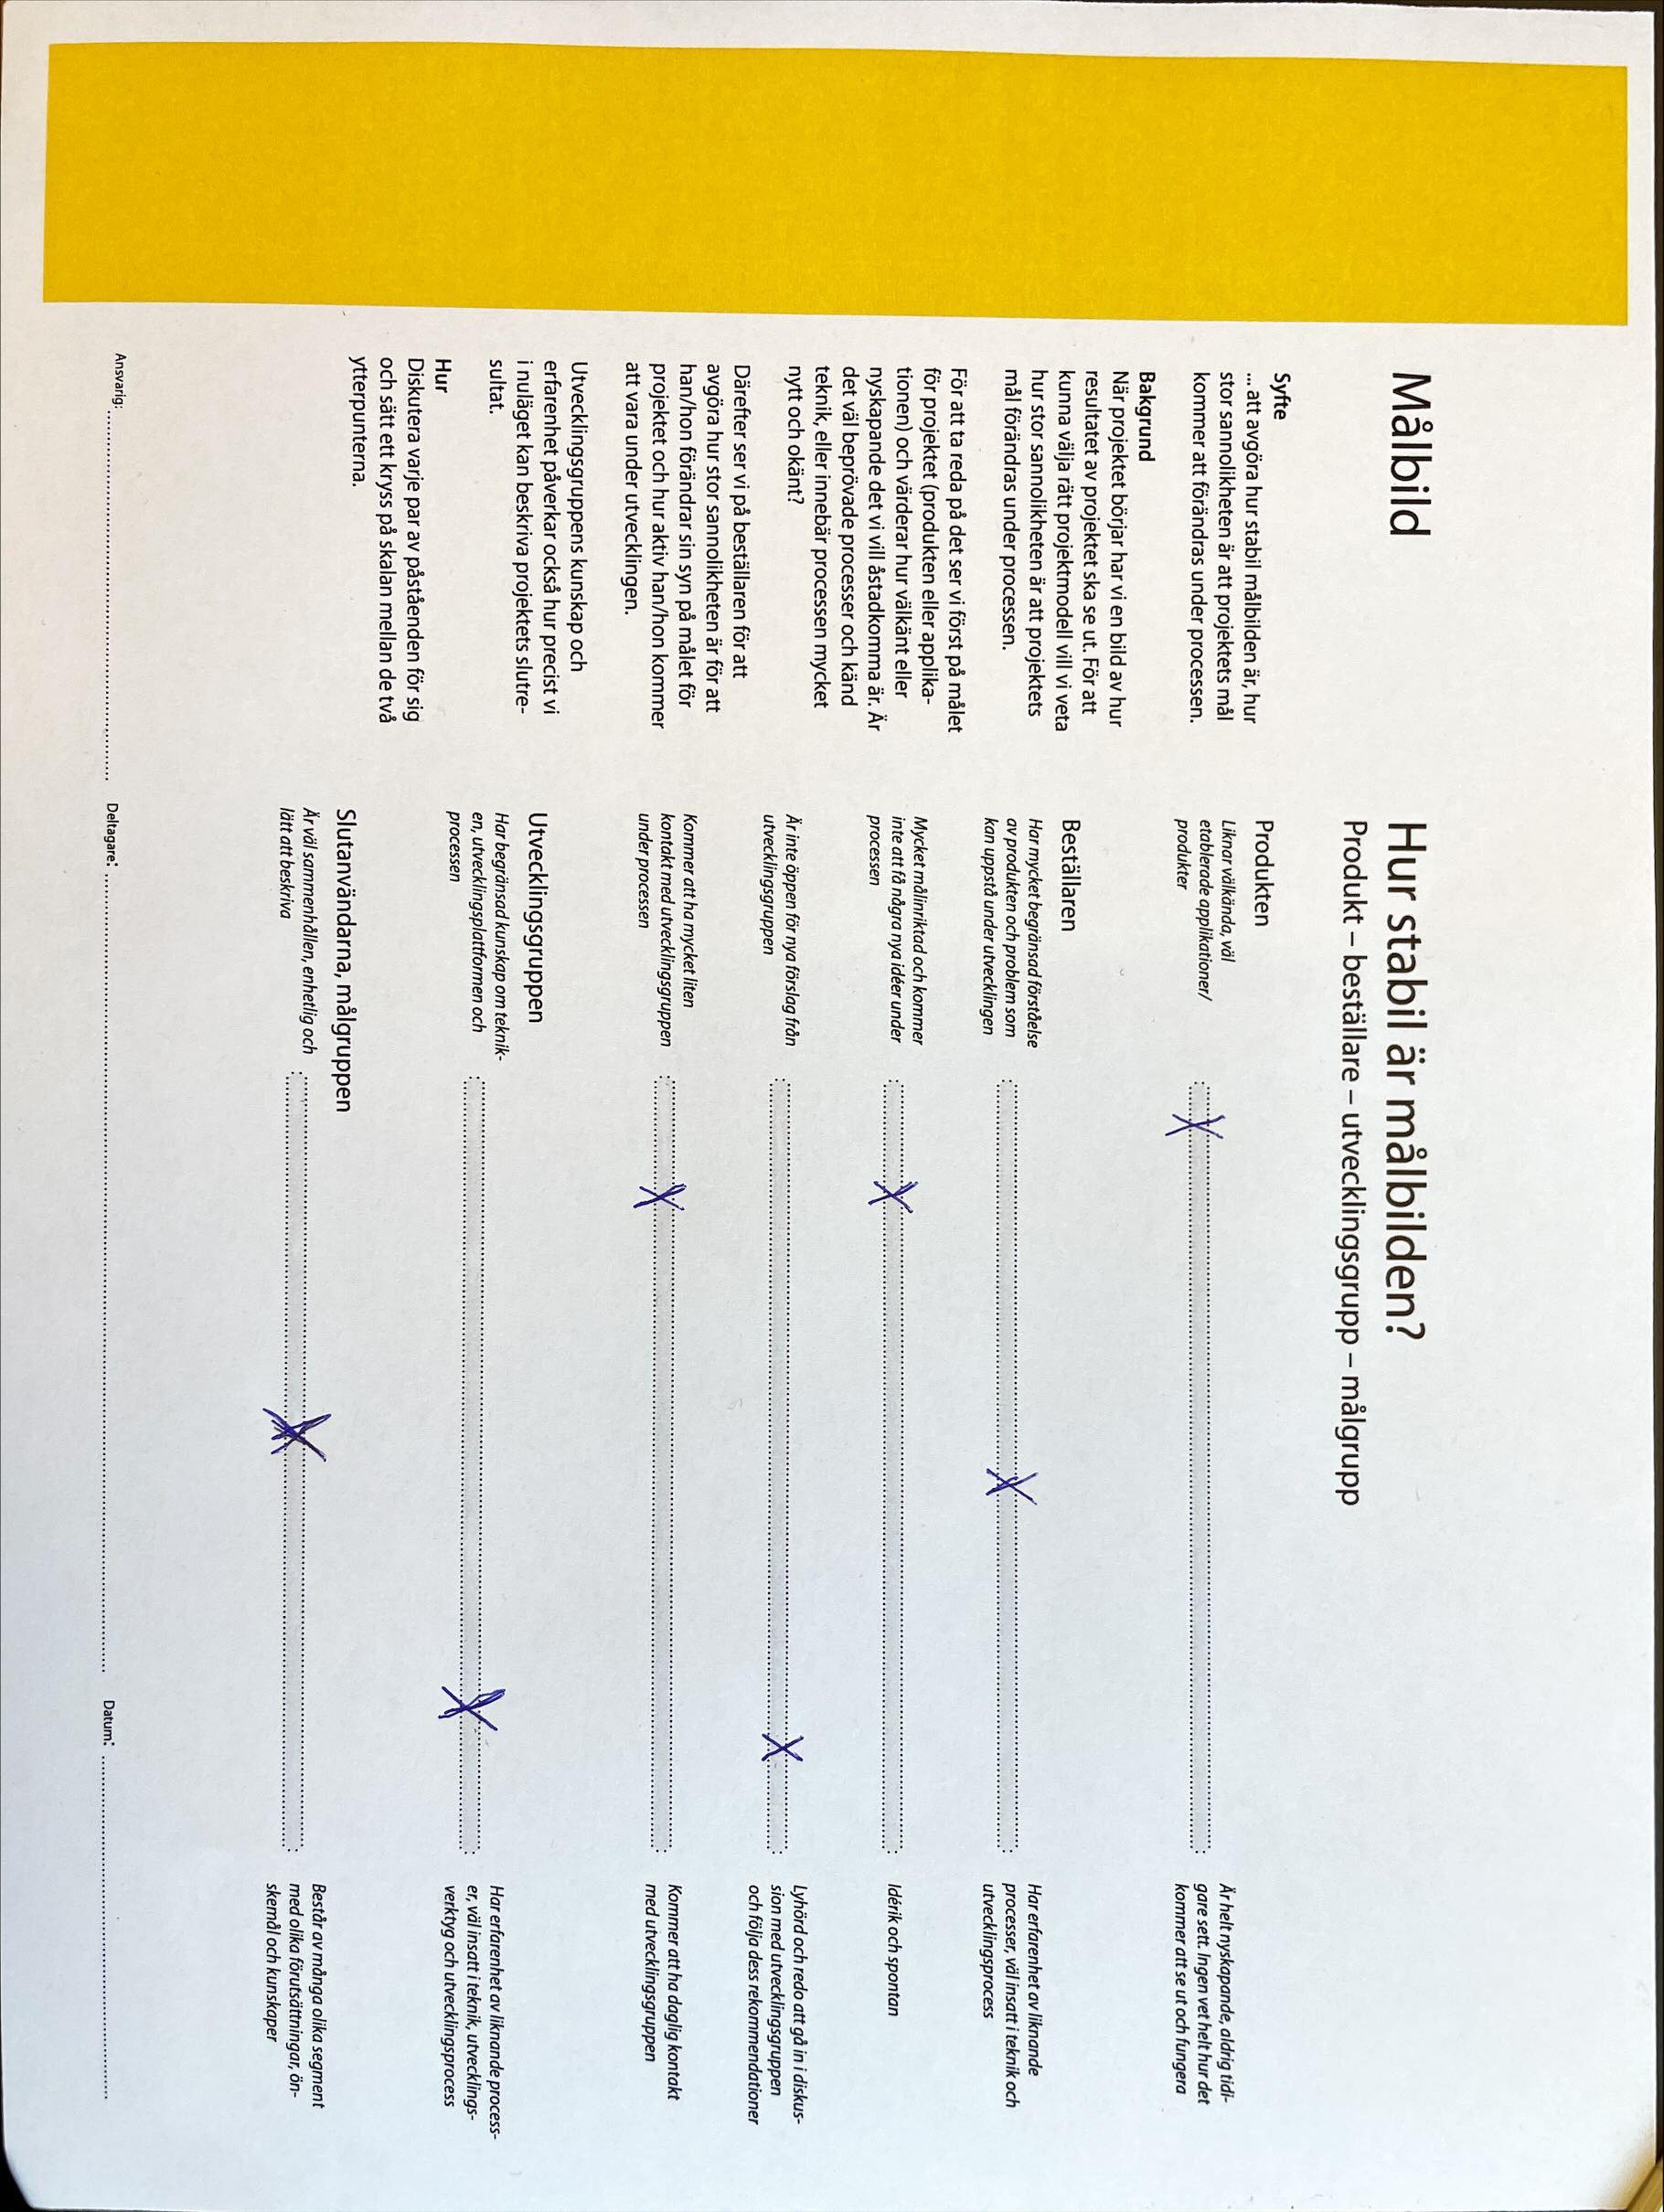
\includegraphics[width = 180px,angle=90]{SM.jpg}
    \caption{Arbetsblad från workshop. Hur stabil är målbilden?}
    \label{fig:Bilaga målbild}
\end{figure}

\begin{figure}[htp]
    \centering
    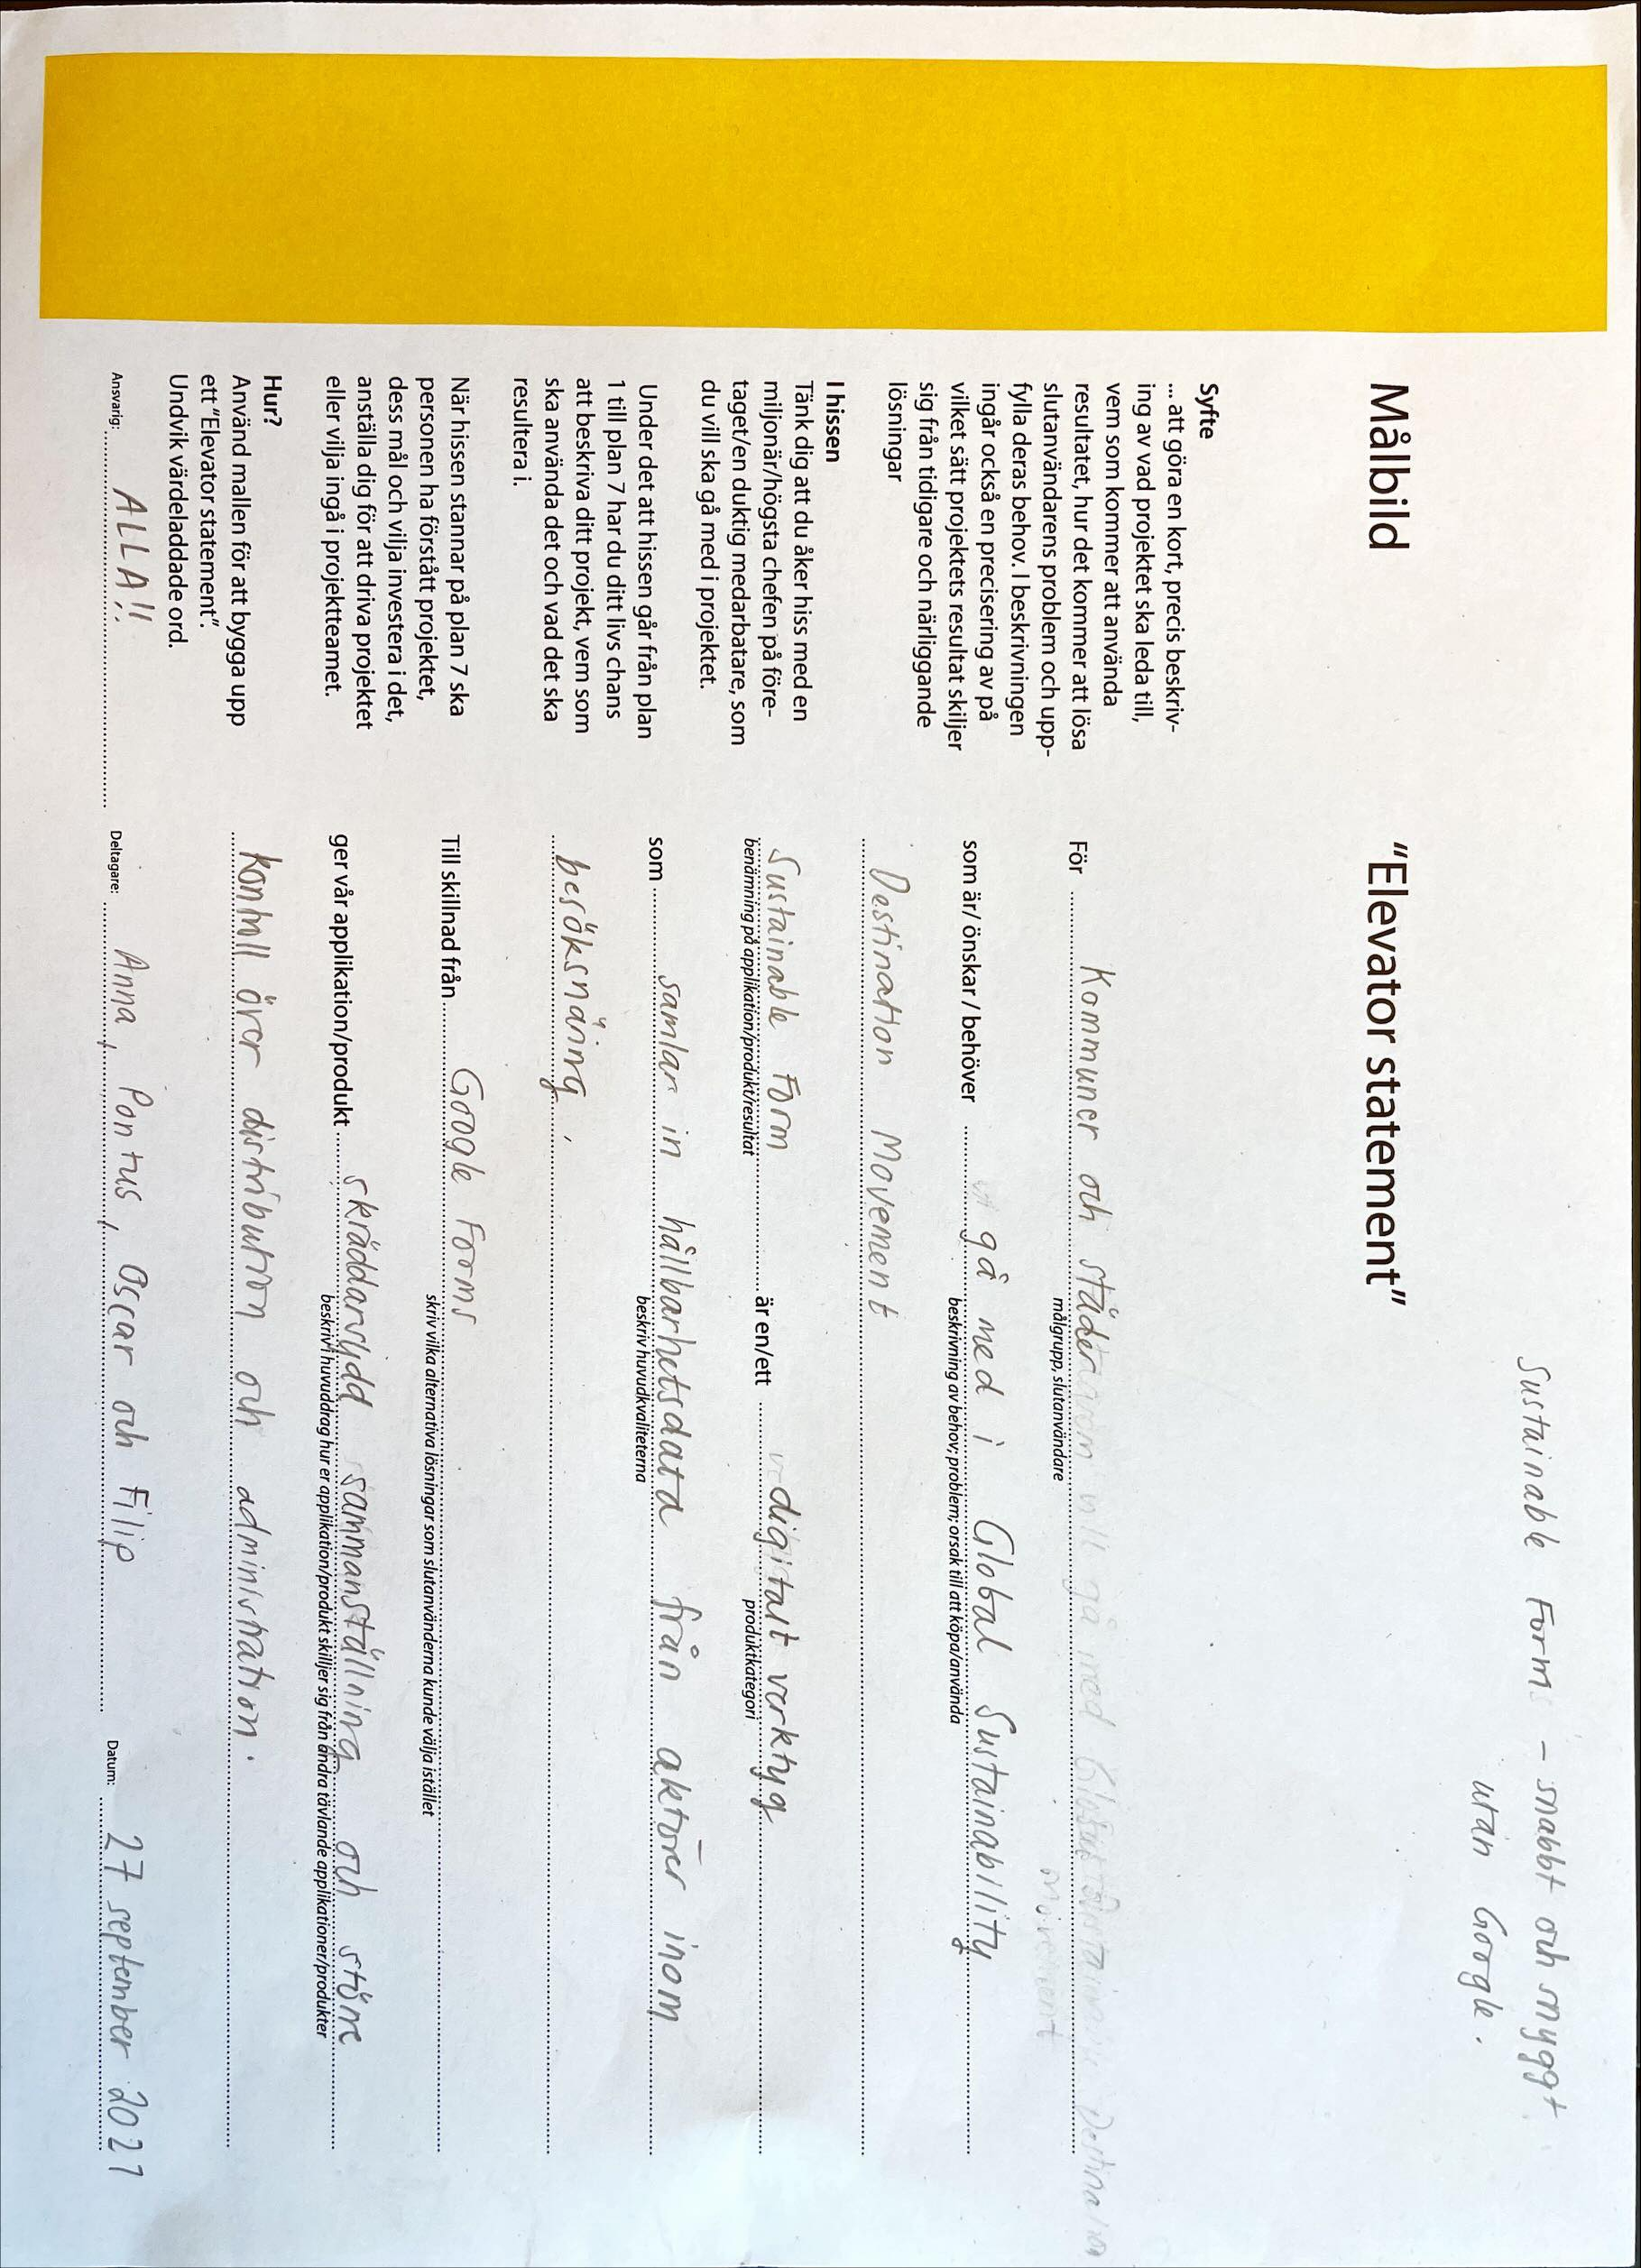
\includegraphics[width = 175px,angle=90]{Elev.jpg}
    \caption{Arbetsblad från workshop. Elevator statement}
    \label{fig:Elevator statement}
\end{figure}

\begin{figure}[htp]
    \centering
    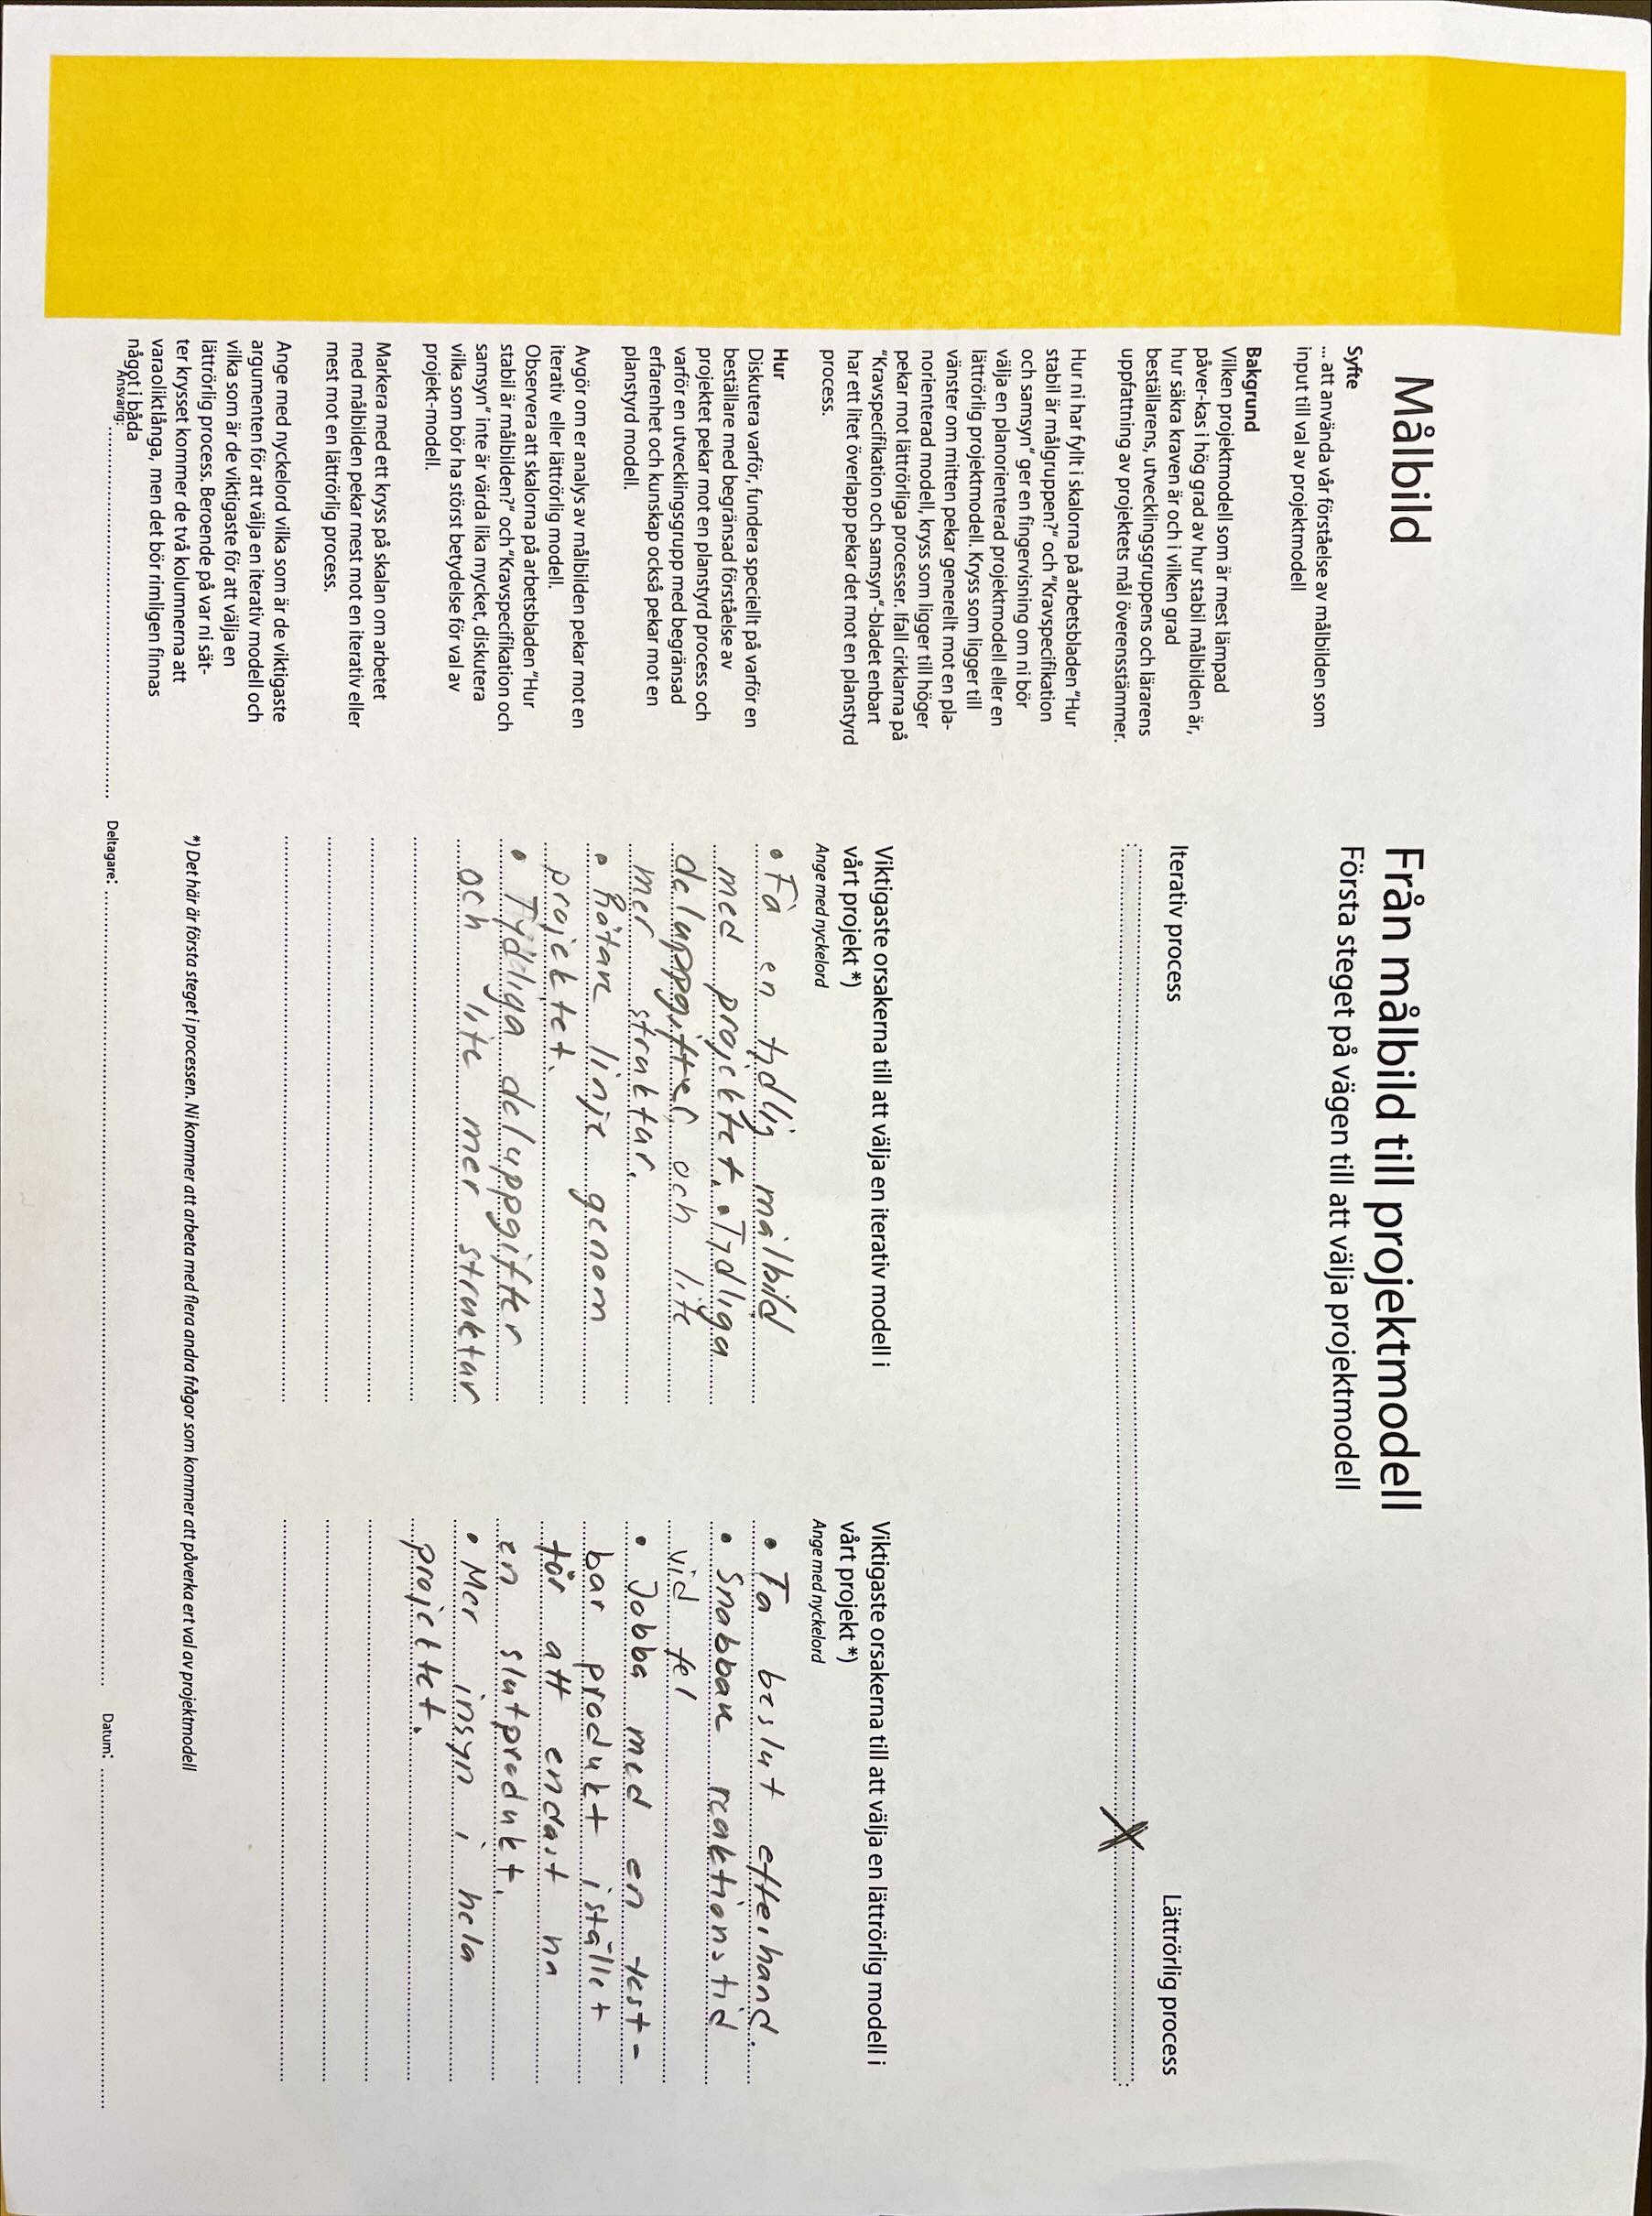
\includegraphics[width = 180px,angle=90]{MP.jpg}
    \caption{Arbetsblad från workshop. Från målbild till projektmodell}
    \label{fig:Bilaga projektmodelll}
\end{figure}





\bibliographystyle{alpha}


\end{document}